\documentclass[11pt,a4paper]{article}
\usepackage[utf8]{inputenc}\usepackage[T1]{fontenc}
\usepackage[margin=1in]{geometry}
\usepackage{amsmath,amssymb,booktabs,graphicx,enumitem,xcolor,parskip,titlesec}
\usepackage[hidelinks]{hyperref}
\graphicspath{{figures/}}
\definecolor{qnavy}{RGB}{20,40,75}\definecolor{qgrey}{RGB}{90,90,90}\definecolor{qred}{RGB}{150,30,30}
\titleformat{\section}{\large\bfseries\color{qnavy}}{\thesection}{0.6em}{}
\begin{document}\thispagestyle{empty}
\noindent
{\large\bfseries\color{qnavy} Report R15 --- Can an H\&E Slide Give You the Methylome?}\\[2pt]
{\color{qgrey}760 matched TCGA lung patients. Partly yes, modestly, and not as a substitute for
the assay.}\\[6pt]
{\color{qred}\textbf{HELD FOR IP --- not for publication pending patent filing.}}\\[4pt]
{\color{qgrey}\rule{\textwidth}{0.4pt}}

\medskip
\noindent 15 August 2026 \quad\textbullet\quad Quantara

\section*{Summary}

The companion-diagnostic product requires a slide to go in and a molecular report to come out.
Everything the programme had built did the two halves separately: biomarkers from slides
(R12/R13), methylation from arrays (R08/R10). This report tests the join, on 760 TCGA patients who
have both Phikon-v2 whole-slide features and 450k methylation --- 413 adenocarcinoma, 347
squamous, across 67 tissue-source sites.

\textbf{H\&E does carry epigenomic information, and it is not merely histological subtype.} Six
fixed, annotation-defined methylation summaries were each predicted from morphology under
site-grouped cross-validation, and all six retain signal after controlling for LUAD-versus-LUSC
status (partial Spearman $\rho$ 0.135--0.244, every one significant, strongest
$p = 9\times10^{-12}$).

\textbf{But it does not replace the assay.} KEAP1 mutation status reaches AUROC 0.664
(95\% CI 0.604--0.722) from the slide, against \textbf{0.910} from the methylation array in R10
--- a shortfall of 0.246. The correlations above, at $\rho \approx 0.2$--0.3, are real
associations, not measurement-grade prediction.

\textbf{A methodological result worth more than either.} The first attempt at this question
returned a clean negative. We supervised the slide embedding on subtype and then asked it about
methylation; it learned nothing useful for the second task and was outperformed by the subtype
label alone --- a 512-dimensional embedding beaten by one binary variable. Training the same
architecture directly on methylation reversed the answer \emph{on the six aggregate targets}.

\textcolor{qred}{\textbf{Corrected 2026-08-17 (R17).}} This paragraph originally read ``\emph{the
negative was an artefact of our own design choice}'' without qualification, and \S5 below claimed
the reversal generally. R17 re-ran the genome-wide scan on the methylation-supervised embedding
and it does \textbf{not} reverse: 83{,}369 CpGs above null against 90{,}137 for the
subtype-supervised embedding, median $\rho$ 0.0073 against 0.0057. The reversal is specific to the
aggregate targets. R17 also shows why --- a patient's \emph{observed} global mean methylation
alone puts 74.7\% of CpGs above null, so five of our six targets being means over large
annotation classes is enough for a representation to learn that one axis while carrying nothing at
CpG resolution.

\section{The site-leakage measurement}

Before any biological claim: this cohort let us isolate how much apparent performance comes from
train and test sharing contributing institutions. Data, architecture, hyperparameters and seeds
were held identical and only the cross-validation partition changed.

\begin{center}
\begin{tabular}{@{}lccc@{}}
\toprule
& \textbf{Site-grouped} & \textbf{Random folds} & \textbf{Inflation} \\
\midrule
LUAD vs LUSC subtype (AUROC) & 0.7992 & 0.9703 & \textbf{+0.1710} \\
KEAP1 mutation (AUROC) & 0.6642 & 0.6660 & +0.0018 \\
\midrule
\multicolumn{4}{@{}l}{\textit{methylation targets (Spearman $\rho$)}} \\
KEAP1 signature & 0.3172 & 0.3927 & +0.0755 \\
global mean & 0.2897 & 0.3680 & +0.0783 \\
CpG island & 0.2182 & 0.3358 & +0.1176 \\
open sea & 0.2868 & 0.3478 & +0.0610 \\
TSS200 promoter & 0.3029 & 0.4212 & +0.1184 \\
gene body & 0.2988 & 0.3577 & +0.0589 \\
\midrule
\textbf{mean methylation inflation} & & & \textbf{+0.0849} \\
\bottomrule
\end{tabular}
\end{center}

Three things follow. The random-fold subtype figure, 0.9703, reproduces an independent
centralized benchmark of 0.970 to within 0.0003, which establishes that the site-grouped numbers
are honest out-of-site performance and not a weak pipeline. Methylation is site-confounded, as
batch effects would predict, but less so than subtype: a naive analysis would have reported
$\rho \approx 0.34$--0.42 where the honest values are 0.22--0.32. And KEAP1 mutation is not
site-confounded at all, because mutation status --- unlike subtype prevalence --- has no
institutional structure to exploit.

\begin{center}
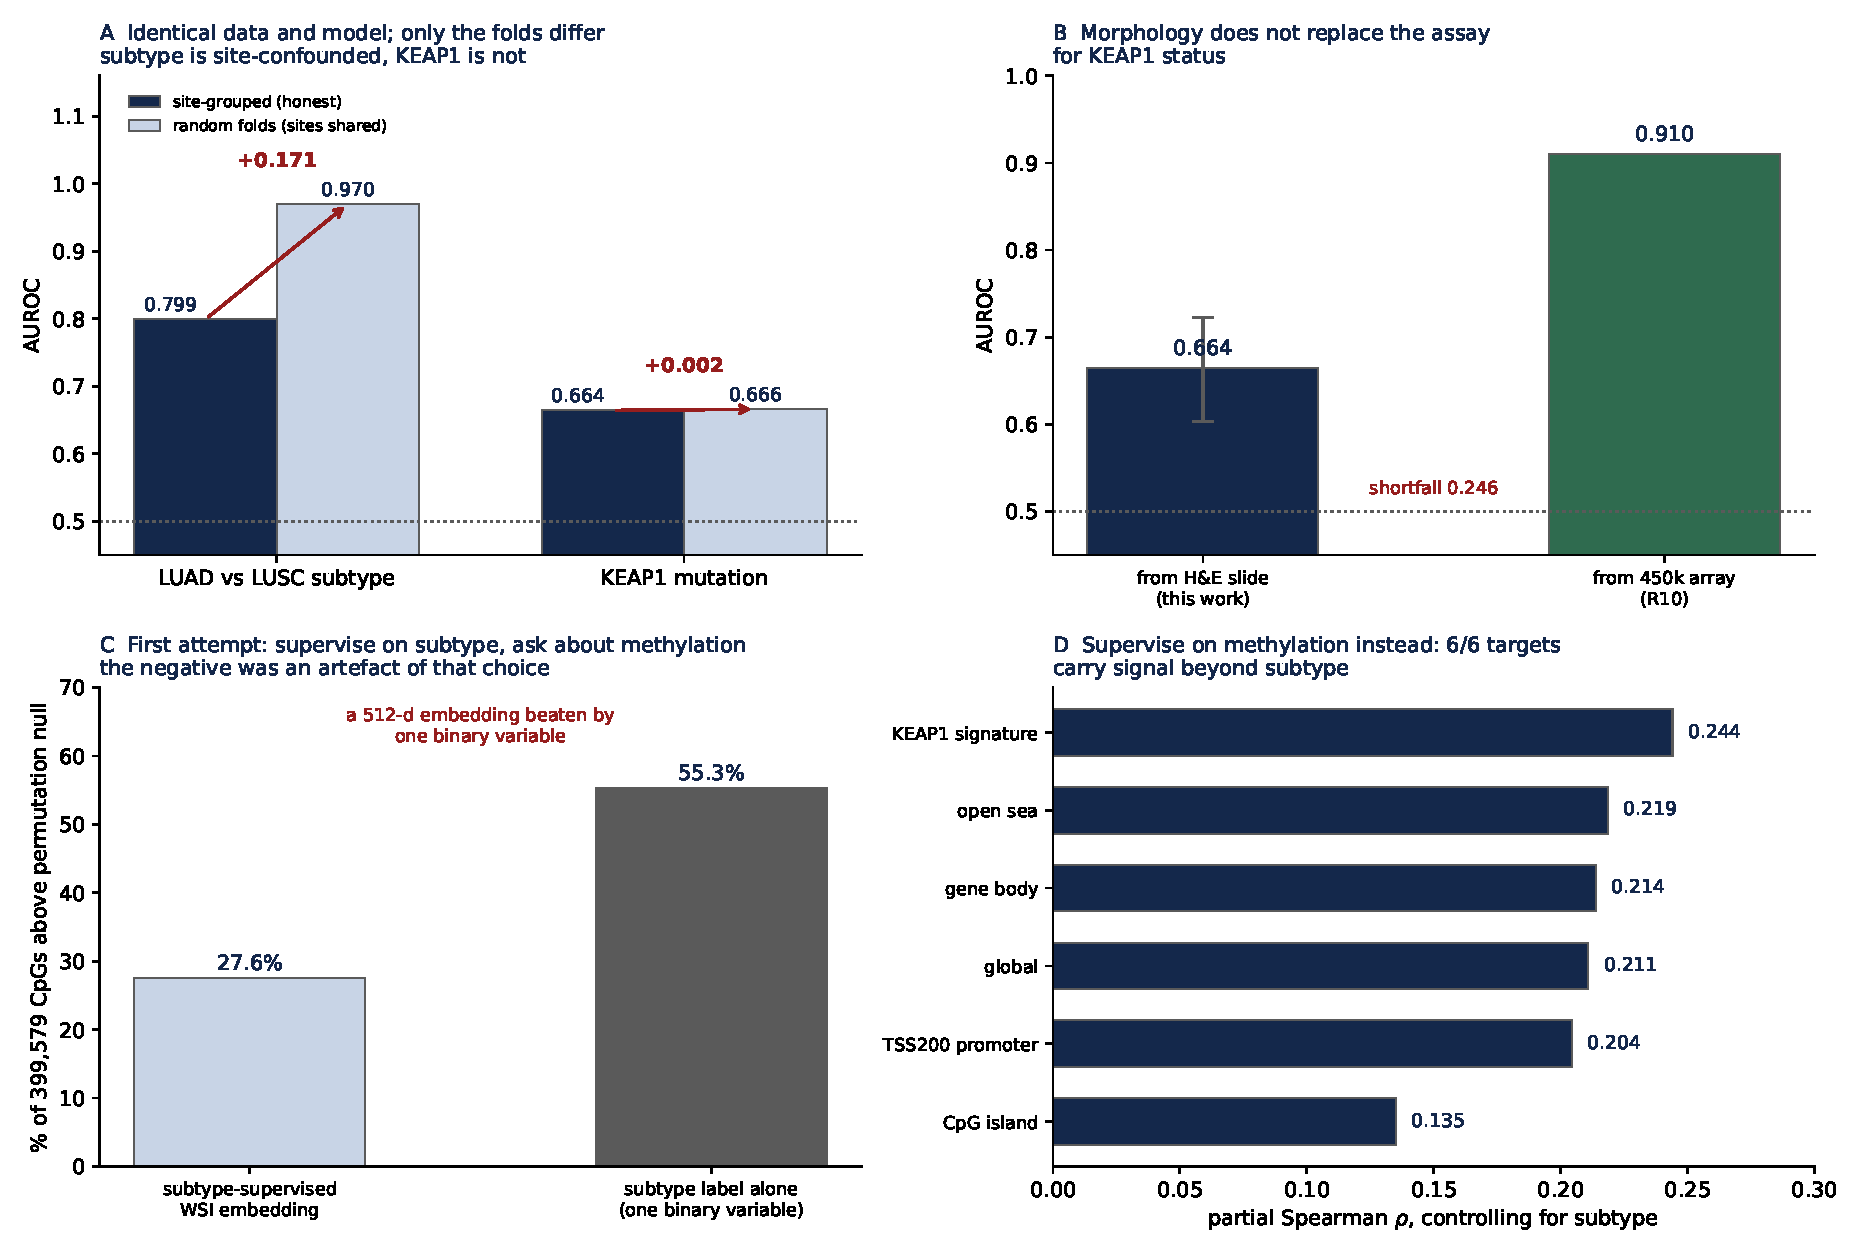
\includegraphics[width=\textwidth]{r15_panels.pdf}
\end{center}
\noindent{\small\color{qgrey}\textbf{A} Fold assignment alone, on identical data and model.
\textbf{B} KEAP1 from slide against KEAP1 from array. \textbf{C} The first, negative answer: a
subtype-supervised embedding loses to the subtype label. \textbf{D} Supervising on methylation
instead --- partial correlations after removing subtype.}

\section{Targets, and why they are defined this way}

Six summaries, each a mean $\beta$ over a \emph{fixed, annotation-defined} probe set. Nothing was
fitted to the data, so there is no selection to argue about:

\begin{center}
\begin{tabular}{@{}lrrl@{}}
\toprule
\textbf{Target} & \textbf{Probes} & \textbf{Mean $\beta$} & \textbf{Definition} \\
\midrule
KEAP1 signature & 115{,}517 & 0.519 & R10's KEAP1-differential probe list \\
global & 399{,}579 & 0.473 & all retained probes \\
CpG island & 134{,}095 & 0.226 & manifest island annotation \\
open sea & 135{,}384 & 0.668 & manifest open-sea annotation \\
TSS200 promoter & \phantom{0}47{,}068 & 0.172 & manifest gene-region annotation \\
gene body & 133{,}165 & 0.628 & manifest gene-region annotation \\
\bottomrule
\end{tabular}
\end{center}

The means sanity-check against known biology --- promoters and islands hypomethylated, open sea
and gene bodies hypermethylated --- which is a cheap check that the matrix is assembled correctly.

\section{Does morphology add beyond histological subtype?}

Subtype is separable from methylation at AUROC 0.955 (R08), so ``H\&E predicts methylation''
could trivially mean ``H\&E predicts subtype, and subtype predicts methylation.'' A pathologist
supplies subtype for free, so the question that matters commercially is whether morphology adds
anything on top of it.

\begin{center}
\begin{tabular}{@{}lrrrr@{}}
\toprule
\textbf{Target} & \textbf{$\rho$ (WSI)} & \textbf{$\rho$ (subtype)} & \textbf{Partial $\rho$} & \textbf{$p$} \\
\midrule
KEAP1 signature & 0.317 & 0.257 & \textbf{0.244} & $9.1\times10^{-12}$ \\
open sea & 0.287 & 0.219 & \textbf{0.219} & $1.1\times10^{-9}$ \\
gene body & 0.299 & 0.270 & \textbf{0.214} & $2.6\times10^{-9}$ \\
global & 0.290 & 0.264 & \textbf{0.211} & $4.3\times10^{-9}$ \\
TSS200 promoter & 0.303 & 0.345 & \textbf{0.204} & $1.3\times10^{-8}$ \\
CpG island & 0.218 & 0.288 & \textbf{0.135} & $1.9\times10^{-4}$ \\
\bottomrule
\end{tabular}
\end{center}

All six. Note that on two targets --- promoter and island --- the subtype label alone
out-predicts the slide, yet the partial correlation remains positive: morphology carries
\emph{different} information rather than more of the same.

\section{The first attempt, and why it was wrong}

Recorded because the sequence is the most transferable thing here.

The first run supervised the attention-MIL on subtype, extracted the 512-dimensional
attention-pooled embedding out-of-fold, then regressed methylation on it. Results: genome-wide
median $\rho = 0.006$; 110{,}212 of 399{,}579 CpGs above the permutation null (27.6\%) against
\textbf{220{,}925 (55.3\%)} for the subtype label by itself; bulk methylation
$\rho = 0.011$, $p = 0.76$; and genomic-context enrichment flat at 0.97--1.01 across island,
shore, shelf and open sea, where R10's KEAP1 phenotype had been strongly structured
(island 0.54, open sea 1.44).

Every one of those readings pointed the same way, and the conclusion --- morphology does not
carry methylation \emph{at all} --- was too broad. The embedding had been optimised to separate two
histological classes, and nothing else was asked of it during training. Supervising on methylation
directly recovered signal \emph{on the six aggregate targets}.

An honest negative therefore needs its supervision examined before it is believed.

\textcolor{qred}{\textbf{Corrected 2026-08-17 (R17).}} Two sentences here originally read
``supervising on methylation directly recovered the signal'' and ``that flatness of genomic
context \ldots was in fact evidence that the representation contained no methylation-relevant
structure to find''. Both are withdrawn. R17 ran this exact scan on the methylation-supervised
embedding: it is not better (83{,}369 above null against 90{,}137), and its genomic context is
still nearly flat --- spread 0.212 against 0.047 --- and tilted the \emph{opposite} way to R10,
with islands enriched at 1.116 where R10 had them depleted at 0.54. So flatness here was not a
diagnostic of the wrong supervision. The genome-wide negative is robust to supervision; see
\texttt{results/R17-percpg-methylation-supervised/}.

\section{Commercial reading}

\begin{itemize}[leftmargin=1.2em,itemsep=3pt]
\item \textbf{A slide cannot replace a methylation assay.} KEAP1 at 0.664 from morphology
against 0.910 from the array. The product is slide \emph{plus} assay, not slide instead of assay.
\item \textbf{Morphology is genuinely informative about the epigenome}, at $\rho \approx 0.2$
beyond subtype. That is a real mechanistic finding and is the patentable content here, but it is
an association, not a measurement.
\item \textbf{This inflation is encoder-specific.} \textcolor{qred}{\textbf{Added 2026-08-17
      (R18).}} The +0.0849 below was re-measured on \texttt{facebook/dinov2-large} with identical
      tiles, folds, architecture and hyperparameters: it becomes \textbf{+0.0004}, with three of the
      six targets moving in the anti-leakage direction. On fraction of remaining headroom, 0.119
      for Phikon-v2 against 0.000. This is not a headroom artefact --- the same comparison shows
      \emph{subtype} leakage reproducing and growing (+0.2034 against +0.1710). So subtype leakage
      is a property of the archive and \emph{methylation} leakage was a property of Phikon-v2
      features. Every methylation-inflation figure in this report should be read as specific to
      this encoder. See \texttt{results/R18-encoder-robustness/}.
\item \textbf{Any naive validation of this capability would have overstated it} by about 0.085
in $\rho$, and by 0.171 in AUROC for subtype. A vendor reporting single-collection
cross-validated numbers is reporting an upper bound.
\end{itemize}


\section{Tumour purity: the most likely benign explanation, tested}

The first version of this report named tumour purity, stromal fraction and proliferation as the
most plausible innocent driver of the association --- all three plausibly move both morphology and
bulk methylation --- and stated that no correction was available. That was premature. TCGA
publishes consensus ABSOLUTE purity estimates, available here for \textbf{741 of 760 patients}
(median purity 0.460).

\textbf{The confound is real.} Purity is strongly associated with observed methylation
($\rho = -0.306$, $p = 1.5\times10^{-17}$ for the KEAP1 signature) and the morphology-derived
predictions do track it ($\rho = -0.218$, $p = 2.2\times10^{-9}$). So the concern was not
hypothetical.

\textbf{Adjusting for it barely moves the result.}

\begin{center}
\begin{tabular}{@{}lrrr@{}}
\toprule
\textbf{Target} & \textbf{Partial $\rho$} & \textbf{+ purity} & \textbf{Change} \\
& (subtype only) & (subtype + purity) & \\
\midrule
keap1\_sig        & 0.252 & 0.221 & -0.031 \\
global             & 0.218 & 0.210 & -0.008 \\
island             & 0.134 & 0.136 & +0.002 \\
opensea            & 0.228 & 0.218 & -0.010 \\
tss200             & 0.210 & 0.190 & -0.021 \\
body               & 0.220 & 0.221 & +0.001 \\
\bottomrule
\end{tabular}
\end{center}

The largest change is the KEAP1 signature, from 0.252 to 0.221. Every target remains significant
(all $p \leq 2.1\times10^{-4}$; four at $p < 10^{-8}$). So morphology carries information about
methylation that is not explained by histological subtype and not explained by how much tumour is
on the slide.

This does not exhaust the confounders --- stromal composition, necrosis and proliferation index are
still unadjusted --- but it removes the one with the strongest prior and the best available
measurement.

\section{Limitations}

\textbf{Association, not mechanism.} Nothing here shows morphology is caused by methylation state
or vice versa. Tumour purity is now adjusted for (\S6) and the association survives; stromal
composition, necrosis and proliferation remain unadjusted.

\textbf{Modest magnitudes.} Partial $\rho$ 0.135--0.244 explains a few percent of variance.
Presented as evidence of information, not of utility.

\textbf{Subtype-supervised embeddings for the first arm only.} The negative in \S5 is bounded to
that design and should not be quoted as a general result about H\&E.

\textbf{One cohort, one encoder, one array platform.} TCGA lung, Phikon-v2, Illumina 450k.
Nothing replicated. The programme has learned (R09) not to assume a replication cohort exists.

\textbf{Six targets, not the full methylome.} Fixed annotation-defined summaries were chosen for
interpretability and leakage-safety. Per-CpG prediction under methylation supervision was not
attempted here --- \textcolor{qred}{it was attempted in R17 (2026-08-17) and is negative}, which
bounds every claim in this report to the aggregate targets.

\textbf{Mean-pooled slide aggregation per patient.} Patients with multiple slides are averaged;
no attempt was made to weight by tumour content.

\section{Reproducing this report}

\begin{itemize}[leftmargin=1.2em,itemsep=1pt]
\item Analysis: \texttt{evidence/m13\_wsi\_to\_methylation.py} (arms and gates);
      \texttt{evidence/mil\_embed.py} (subtype-supervised MIL);
      \texttt{evidence/mil\_meth.py} and \texttt{mil\_meth\_random.py} (methylation-supervised,
      site-grouped and random arms)
\item Config hash, written before any outcome was read:
      \texttt{3d8b9658f679e069\ldots2c5a5ef3}
\item \texttt{evidence/meth\_leakage\_arm.json} --- the grouped/random comparison for all six
      targets
\item \texttt{evidence/per\_cpg\_rho\_\{grouped,null,subtype\_only\}.npy} --- all 399{,}579
      per-CpG correlations from the first arm
\item Figure: \texttt{python3 make\_figure.py}
\end{itemize}

\end{document}
